\documentclass[11pt]{article}

\usepackage[a4paper]{geometry}
\usepackage[warn]{mathtext}
\usepackage[T2A]{fontenc}
\usepackage[utf8]{inputenc}
\usepackage[russian,english]{babel}

\usepackage{amssymb,amsmath}

\usepackage{shorttoc}
\usepackage{hyperref}

\usepackage{graphicx}

\usepackage{indentfirst}

\newenvironment{docs}
{\par\begin{tabular}{|p{.95\textwidth}}\raggedright}
{\end{tabular}\\[1.0ex]}

\renewcommand*\contentsname{Contents (detailed)}

% \usepackage{rumathbr}
% \usepackage{std}

\widowpenalty=500
\clubpenalty=500

\begin{document}
    \setcounter{page}{0}

    \title{\textbf{Intermediate coursework report}}
    \author{Goncharov Vladimir}

    \thispagestyle{empty}

    \begin{center}
    ~\\[10ex]
    {National Research University ``Higher School of Economics''}\\
    Faculty of Computer Science\\
    Applied mathematics and informatics\\[15.0ex]
    {\LARGE\bf Intermediate coursework report}\\[4.0ex]
    {\Large\bf Implement autonomous navigation system for quadcopter capable of tracking clearly marked objects}\\[4.0ex]
    Vladimir Goncharov, [Peter Kuznetsov?], [Dmitry Dubov?]\\
    research advisor Bruno Bauwens\\[4.0ex]
    \end{center}

    \newpage

    % \pdfbookmark[1]{Contents}{toc}
    % \shorttoc{Contents}{1}

    \tableofcontents

    \newpage

    \section{Introduction}

    The goal of the project is to implement relatively simple
    well documented control system for ARdrone 2 quadrocopter
    capable of tracking a special mark or an object that is known before launch.

    We also aim two additional targets: first is to provide base for further
    more complex research, and second is to prepare well structured material
    for fast mastering ROS and additional tools that are required to control
    the drone so that those who have no experience with this technology
    can focus on creating something new rather than dealing with
    implementation details.

    In this intermediate report we provide information about current project
    status and general overview of tools and methods
    that are used or will be used to implement final algorithm.

    \section{Technologies~used}

    We will now provide brief description of technologies used.
    
    A more detailed overview is available in the sections
    below or in the respective documentation pages~\cite{ROSsite, OpenCVsite}.

    Robot Operating System (ROS) package is used as a main framework.
    ROS is an open-source C++ library for implementing efficient modular
    distributed yet simple systems. It comes with many useful built-in
    features which makes development easier.

    To communicate with drone the ``ardrone-authonomy''
    package is used~\cite{ArdroneAuthonomy}.
    This package is build on top of the ROS. It provides simple interface for
    the drone's manipulation, including odometry~--- coordinates of the drone
    based on the accelerometers data.

    For image processing open-source cumputer vision library (OpenCV) is used.
    
    Python programming language bindings are available for both ROS
    and OpenCV. They are used when no complex computation methods are required.
    Python code is easier to read and easier to write.
    Thus it is possible to combine Python and C++ to acieve flexibility,
    computational efficiency, and simplicity at the same time.

    For user interface drawing the PyQt~\cite{PyQt} library is used.

    In addition to the tools and packages listed above,
    more complex systems can be included to the project in the later stages.

    \section{ROS~overview}

    As it was mentioned before, ROS allows easy implementation
    of distributed systems.

    The key to the simplicity is ``modularity'' approach.
    Any ROS application is a set of many executables called ``nodes''.
    Nodes are connected into a single network.
    This approach allows to avoid single monolithic programms
    by splitting them into separate interchangeable subprogramms.

    We will briefly describe how nodes are communicating.
    For more detailed overview refer to the documentation~\cite{ROSsite, ArdroneAuthonomy, roslaunch, rostopic}

    \paragraph{Launch} Nodes can be launched with a single command:

    \noindent{\tt rosrun package\_name node\_name}.

    However, this is not convenient for launching projects with big
    amount of nodes.

    To solve this problem, we one can use the ``roslaunch''~\cite{roslaunch} commandline tool
    which comes with ROS. This tool reads launch config file (typically an
    XML file) and launches all infrastructure as described in that config.

    We have several launch files defined in this project. One simply
    launches the drone's driner, anuther one launches CV system with
    webcamera as a video source, and the other launches the entire system.

    \paragraph{Communication} Nodes communicate with the others by sending messages
    through the ROS master server and by listening for other messages
    to arrive.

    To make the system more organized, all messages are systematized into
    channels called ``topics''. This means that nodes doesn't need to listen
    for all messages trying to segregate those that are usefull for this node.
    ROS master server will do this job for us.

    This can be treated as a big forum where all messages are grouped
    by subjects (that is, subjects are topics in ROS terminology).
    Each topic contains messages of a particular type
    with a particular subjects. This type restriction comes with limitation of
    the C++ programming language, which is statically typed.

    For example, the topic called ``/rosout'' is a text topic for debug
    messages; the topic called ``/ui/image'' is an image data topic used
    in the system for sharing video data.

    So, each node can publish a message to any topic.

    At the same time each node can subscribe to any available topic.
    After a node is subscribed to a topic, it will instantly receive
    any message published to that topic.

    This makes nodes interchangeable. Even more, for each node we can remap
    names of topics so that nodes can use any convenient name without care
    for global names.

    For example we have an user interface (UI) node which shows the video
    stream located in ``/ui/image'' topic.

    We also have drone's driver which publishes the drone's video stream to\\
    ``ardrone/image\_raw'', ``ardrone/front/image\_raw'',
    and ``ardrone/bottom/image\_raw'' topics.

    Additionally we have a ``webcam\_stream'' node which
    can capture webcamera stream
    and publish it to the ``/webcam/image'' topic.

    This three nodes described abude use different topic names for video
    streaming. However, we can combine these nodes by rerouting their topics.

    Indeed, launching

    \noindent{\tt rosrun ardrone\_autopilot interface.py}\\
    \noindent{\tt rosrun ardrone\_autopilot webcam\_stream.py /webcam/image:=/ui/image}

    will make ``webcam\_stream'' node to publish its camera stream to the
    ``/ui/image'' topic so that UI node can show it.

    On the other hand, launching drone's driver
    with the same UI node as

    \noindent{\tt rosrun ardrone\_autopilot interface.py /ui/image:=ardrone/image\_raw}
    \noindent{\tt roslaunch ./src/ardrone\_autopilot/launch/driver.launch}

    will cause UI node to work with drone's camera.

    As you can see, one can easily change ``webcam\_stream'' node and the
    drone's driver camera node. This is exactly what we call ``modularity''.

    It's especially useful for offline debugging of the project when there's
    no need to connect to the real drone.
    For example, working with CV system will not require anything but a
    video stream. Thus we may replace the video stream sent by the real drone
    with a single ``webcam\_stream'' node.

    \paragraph{Video streaming limitation} Video streaming produces high channel load.
    Therefore one should use ROS topics with caution
    in order to not overload the network.

    So far we have four image topics and we see no apparent problems.
    However we've seen bandwidth impact while transmitting more than six topics:
    the entire system becomes slow, time lags are sufficiently big.

    This was just lab test, but other people reported the same issues~\cite{BandwidthProblems}
    (There are more; I'll add links in the final report).

    Thus it is resonable to implement all CV logic in one node rather than
    spliting simple operations into different nodes.

    Topics can be debugged vith ``rostopic''~\cite{rostopic} commandline tool
    which comes with ROS.

    \section{Computer~vision}

    \section{Odometry~systems}

    \section{Drone~control}

    \section{Current~and~planned~project~structure}

    We have three main parts of the project.

    First part is a target recognition system based on computer vision (CV)
    algorithms.
    We already have it in a simple form, but in the current state it's not yet
    ready to operate drone effectively.

    Depending on the target complexity and the environment conditions
    we may use various algorithms. Several choices are possible, such as
    simple shape and pattern recognition
    (e.g. built-in {\tt cvFindChessboardCorners} OpenCV method),
    or more advanced, like the old-good Viola-Jones
    method~\cite{HaarCascade}.

    Second part is the information processor. It is needed to estimate the
    drone's position in a global coordinate frame so that we could determine
    the target location regardless of the position of the drone.

    It is critical to calculate this data as accurate as possible.
    Sending commands to the drone generates a positive feedback.
    Indeed, by sending ``froward'' command we will
    change the drone's pitch. This change will make the CV system report
    the target position changes even though the actual position
    remains the same.

    We need to track drone's position in order to eliminate this feedback.

    In the initial stages we plan to use odometry data provided by drone's
    driver. If we are not satisfied with this data, we can try detecting
    drone movements by using SLAM\footnote{Simultaneous
    localization and mapping} algorithms. These algorithms yilded
    good results in similar situations~\cite{PATM, PATMonline}.

    And the third part is the actual drone's control system.
    We will need to use those CV and odometry data provided by the two parts
    described above to yield commands for the drone.
    We have some drafts in this parts although we are not yet ready to
    present them.

    The above parts are implemented as a separate nodes.
    So far we have four nodes implemented.

    The first one is called ``UI node''. It is needed to provide user interface
    so that one can control programm.
    It shows video stream from the camera and all debugging info.
    This node relies on PyQt~\cite{PyQt} for drawing the interface.

    Another one, which is called ``commands commutator'',
    is needed for switching commands source.
    For example we may switch between the keyboard input, the joystick input, 
    and the autopilot commands flow.

    The CV module will recognize target (first part) and the Control module will
    translate tagret's coordinates from the local coordinate frame to the
    global one and work out actual commands which will be sent to the drone
    (second and third parts).

    We've decided to merge second and third parts in order to elliminate
    time lag produced by transferring information through the master server.

    These CV and Control nodes are present in the project code.
    They are working as a data relays, though.

    \begin{figure}[ht!]
        \noindent\centering
            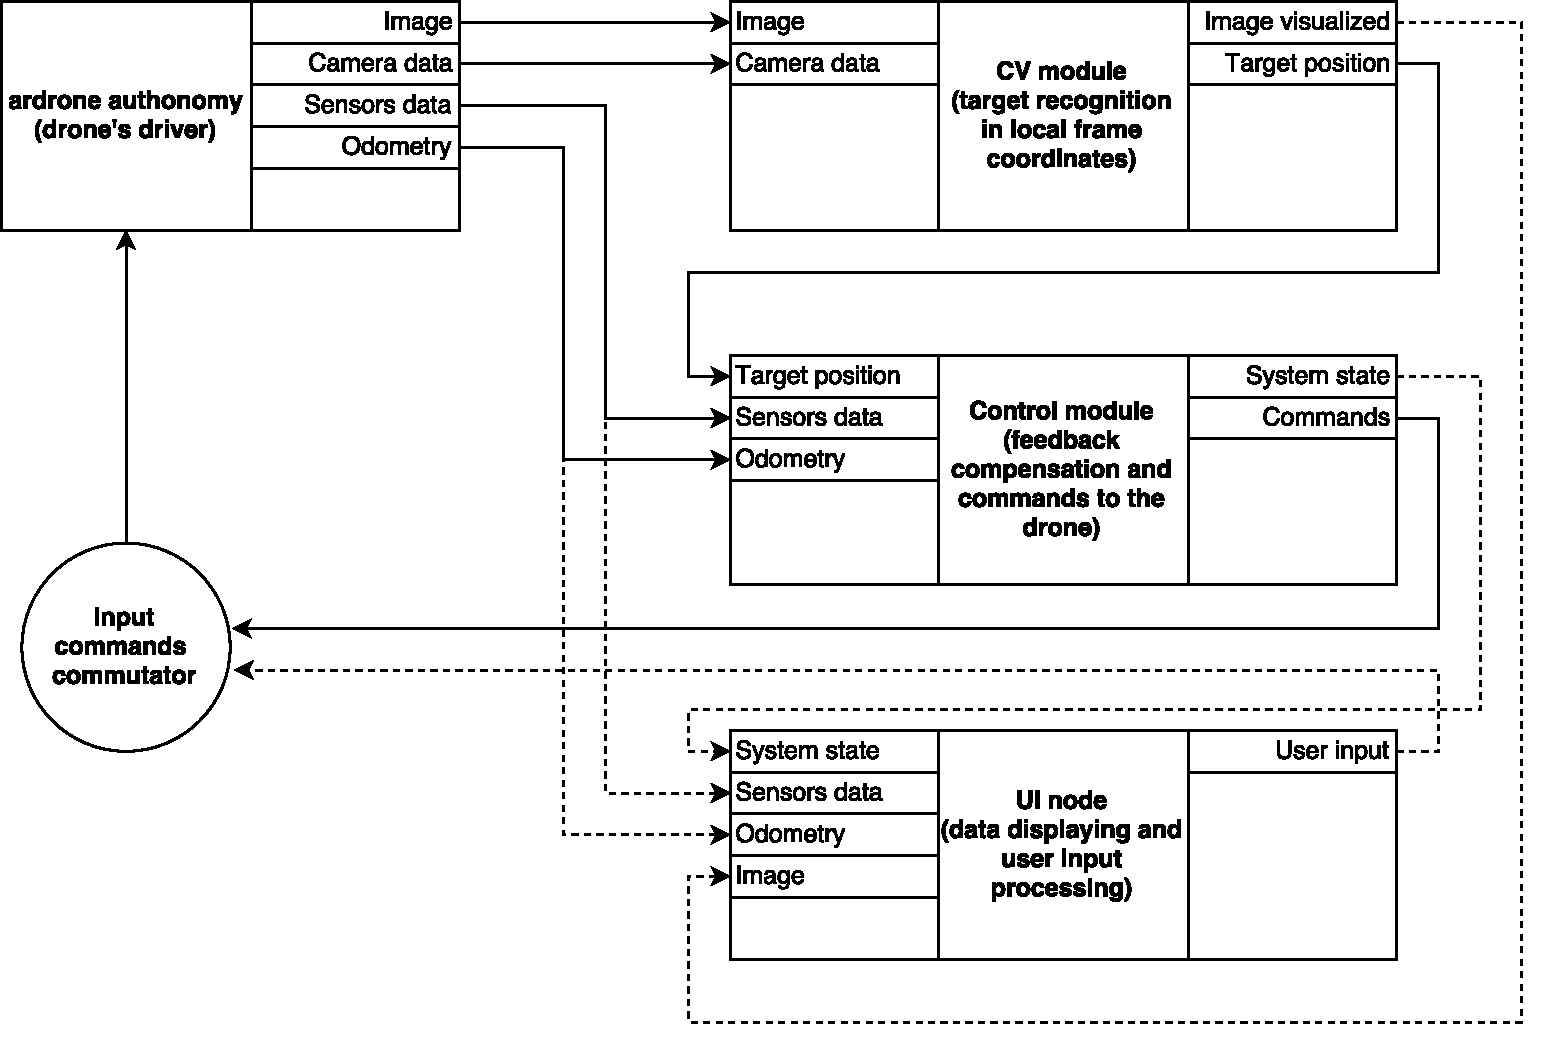
\includegraphics[width=\textwidth]{nodes.pdf}
        \caption{Project dataflow graph}
        \label{fig:DFGraph}
    \end{figure}

    Figure~\ref{fig:DFGraph} shows current project structure.
    CV and Logic modules are produces no effect on the system for now.

    We may need to add one more node in case if we use external odometry
    systems (SURF and co.).

    \newpage

    \setcounter{page}{1}
    \pagenumbering{roman}

    \begin{thebibliography}{9}

    \bibitem{ROSsite}
        ROS documentation is currently available at \\
      http://www.wiki.ros.org

    \bibitem{ArdroneAuthonomy}
        Ardrone Authonomy repository and documentation is currently available at \\
      http://www.ardrone-autonomy.readthedocs.org/en/latest/ \\
      https://github.com/AutonomyLab/ardrone\_autonomy

    \bibitem{OpenCVsite}
        OpenCV documentation is currently available at \\
      http://www.opencv.org/documentation.html

    \bibitem{PyQt}
        PyQt is a library for implementing user interface systems.
        PyQt is a Python wrapper for the Qt library.

        Information about PyQt is currently available at \\
        https://www.riverbankcomputing.com/software/pyqt/intro

    \bibitem{HaarCascade}
        Paul Viola, Michael Jones, \emph{Rapid object detection using a boosted cascade of simple features, Computer Vision and Pattern Recognition}, 2001

    \bibitem{SURF}
        Herbert Bay, Andreas Ess, Tinne Tuytelaars, Luc Van Gool, \emph{Speeded Up Robust Features}, ETH Zurich, Katholieke Universiteit Leuven


    \bibitem{roslaunch}
        Roslaunch is a tool for launching ROS application.
        Its documentation is currently available at \\
        http://wiki.ros.org/roslaunch

    \bibitem{rostopic}
        Rostopic is a tool for displaying debug information about ROS Topics.
        Its documentation is currently available at \\
        http://www.wiki.ros.org/rostopic

    \bibitem{BandwidthProblems}
       http://www.ros-users.122217.n3.nabble.com/Is-ROS-limiting-channel-bandwidth-over-network-td2648257.html

    \bibitem{PATM}
        Georg Klein, David Murray, \emph{Parallel Tracking and Mapping for Small AR Workspaces} Active Vision Laboratory Department of Engineering Science University of Oxford
    
    \bibitem{PATMonline}
        PATM implementation is currently available as ROS package at \\
        http://www.wiki.ros.org/tum\_ardrone
        
    \bibitem{mvSLAM}
        Somkiat Wangsiripitak, David W Murray, \emph{Avoiding moving outliers in visual SLAM by tracking moving objects}
        
    \bibitem{mvSLAM2}
        Abhijit Kundu, C. V. Jawahar and K Madhava Krishna, \emph{Realtime Moving Object Detection from a Freely Moving Monocular Camera}
    
    \bibitem{RAPID}
        Chris Harris, Carl Stennett, \emph{RAPID - A Video Rate Object Tracker} Roke Manor Research Ltd., Roke Manor, Romsey, Hampshire, England
    
    \bibitem{mvSLAM3}
        Wei Tan, Haomin Liu, Zilong Dong, Guofeng Zhang, Hujun Bao, \emph{Robust Monocular SLAM in Dynamic Environments}, State Key Lab of CAD\&CG, Zhejiang University

    \end{thebibliography}

\end{document}
